\subsection{Liên kết, hệ tọa độ và số bậc tự do}

\begin{frame}{Liên kết Holonomic và phi Holonomic}
\vspace{-4mm}
\begin{columns}
\column{0.5\textwidth}
    \begin{itemize}
        \item\textbf{Liên kết Holonomic}
    \end{itemize}
    \begin{equation}
        f \left( \mathbf{q}, t \right) = 0.
    \end{equation}
    \vspace{-9mm}
    \begin{figure}
        \centering
        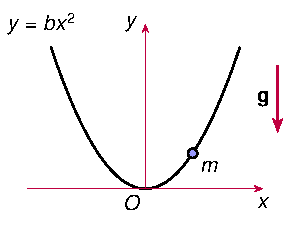
\includegraphics[width=0.8\textwidth]{Figures/Parabol_motion.pdf}
        \vspace{-6mm}
        \caption{Một hạt chuyển động trên bề mặt parabol dưới tác dụng của trọng lực.}
    \end{figure}

\column{0.5\textwidth}
    \begin{itemize}
        \item\textbf{Liên kết phi Holonomic}
    \end{itemize}
    \begin{equation}
        f \left( \mathbf{q}, \dot{\mathbf{q}}, t \right) = 0.
    \end{equation}
    \vspace{-9mm}
    \begin{figure}
        \centering
        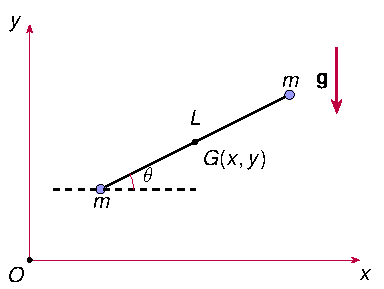
\includegraphics[width=0.8\textwidth]{Figures/NonHolonomic_example.pdf}
        \vspace{-2mm}
        \caption{Một thanh chuyển động dưới tác dụng của trọng trường.}
    \end{figure}
\end{columns}
\end{frame}

\begin{frame}{Bậc tự do}
    \vspace{-4mm}
\begin{columns}
\column{0.6\textwidth}
    \begin{itemize}
        \item \textbf{Số bậc tự do} \\
        \(= \) số tọa độ suy rộng \( - \) số liên kết.
    \end{itemize}
    \begin{itemize}
        \item Ví dụ: con lắc kép.
    \end{itemize}
    \textbf{Cách 1:} Sử dụng 4 tọa độ suy rộng \(\left( x_A, y_A, x_B, y_B \right)\).

    Các liên kết:
    \vspace{-2mm}
    \begin{align}
        f_1 &= x_A^2 + y_A^2 - l_1^2 = 0, \\
        f_2 &= \left( x_B - x_A \right)^2 + \left( y_B - y_A \right)^2 - l_2^2 = 0.
    \end{align}

    \vspace{-2mm}
    Suy ra số bậc tự do: \(4 - 2 = 2\)

    \textbf{Cách 2:} Sử dụng 2 tọa độ suy rộng \(\left( q_1, q_2 \right)\), không có liên kết giữa \(q_1\) và \(q_2\).

    Suy ra số bậc tự do: \(2 - 0 = 2\)

    
\column{0.4\textwidth}
    \begin{figure}
        \centering
        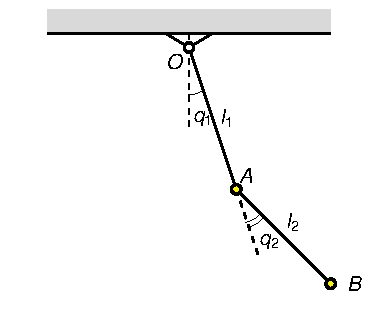
\includegraphics[width=0.9\textwidth]{Figures/Double_pendulum.pdf}
        \caption{Con lắc kép.}
    \end{figure}
\end{columns}
\end{frame}

\subsection{Jacobian và liên hệ vận tốc giữa các hệ tọa độ}

\begin{frame}{Robot Scara 4 bậc tự do}
    \begin{columns}
        \column{0.5\textwidth}
        \begin{itemize}
            \item Robot Scara có 4 bậc tự do biểu diễn qua các tọa độ: \( q = [q_1, q_2, q_3, q_4]^T \).
            \item 3 khớp quay: \(q_1\), \(q_2\), \(q_4\).
            \item 1 khớp tịnh tiến: \(q_3\).
        \end{itemize}
        \begin{figure}
            \centering
            \includegraphics[width=0.8\linewidth]{Figures/Scara_xOz.png}
            \caption{Mặt cắt phương xOz của Robot Scara.}
            \label{fig:Scara_xOz}
        \end{figure}
        \column{0.5\textwidth}
        \begin{figure}
            \centering
            \includegraphics[width=0.8\linewidth]{Figures/Scara_xOy.png}
            \caption{Mặt cắt phương xOy của Robot Scara.}
            \label{fig:Scara_xOy}
        \end{figure}
    \end{columns}
\end{frame}

\begin{frame}{Ma trận Jacobian và liên hệ vận tốc giữa các tọa độ}
    \begin{columns}
        \column{0.5\textwidth}
            \begin{itemize}
                \item Cho hai hệ tọa độ: \( q = \left[ q_1, q_2, q_3 \right]^T\) và \( P = \left[ x, y, z \right]^T\).
                \item Dựa vào phép đạo hàm toàn phần
            \end{itemize}
            \begin{align}
                \dot{x} &= \dfrac{\partial x}{\partial q_1} \dot{q}_1 + \dfrac{\partial x}{\partial q_2} \dot{q}_2 + \dfrac{\partial x}{\partial q_3} \dot{q}_3, \\
                \dot{y} &= \dfrac{\partial y}{\partial q_1} \dot{q}_1 + \dfrac{\partial y}{\partial q_2} \dot{q}_2 + \dfrac{\partial y}{\partial q_3} \dot{q}_3, \\
                \dot{x} &= \dfrac{\partial x}{\partial q_1} \dot{q}_1 + \dfrac{\partial z}{\partial q_2} \dot{z}_2 + \dfrac{\partial z}{\partial q_3} \dot{q}_3.
            \end{align}
        \column{0.5\textwidth}
            \begin{itemize}
                \item Ma trận Jacobian
            \end{itemize}
            \begin{equation}
                J = \left[ \begin{array}{ccc}
                    \dfrac{\partial x}{\partial q_1} & \dfrac{\partial x}{\partial q_2} & \dfrac{\partial x}{\partial q_3} \\
                    \dfrac{\partial y}{\partial q_1} & \dfrac{\partial y}{\partial q_2} & \dfrac{\partial y}{\partial q_3} \\
                    \dfrac{\partial x}{\partial q_1} & \dfrac{\partial z}{\partial q_2} & \dfrac{\partial z}{\partial q_3}
                \end{array} \right].
            \end{equation}
            \begin{itemize}
                \item Ứng dụng: \(\dot{P} = J \dot{q}\).
            \end{itemize}
    \end{columns}
\end{frame}

\begin{frame}{Ma trận Jacobian và liên hệ vận tốc giữa các tọa độ}
    \begin{itemize}
        \item Ứng dụng cho Robot Scara.
    \end{itemize}
            \begin{align}
                \dot{x} &= \left[ -a_1 \sin \left( q_1 \right) - a_2 \sin \left( q_1 + q_2 \right) \right] \dot{q}_1 - a_2 \sin \left( q_1 + q_2 \right) \dot{q}_2, \\
                \dot{y} &= \left[ a_1 \cos \left( q_1 \right) + a_2 \cos \left( q_1 + q_2 \right) \right] \dot{q}_1 - a_2 \cos \left( q_1 + q_2 \right) \dot{q}_2, \\
                \dot{z} &= -\dot{q}_3.
            \end{align}
    \begin{itemize}
        \item Tính độ lớn vận tốc
    \end{itemize}
    \begin{equation}
        v^2 = \dot{x}^2 + \dot{y}^2 + \dot{z}^2
        = \left[ \begin{array}{ccc}
            \dot{x} & \dot{y} & \dot{z}
        \end{array} \right]
        \left[ \begin{array}{c}
            \dot{x} \\
            \dot{y} \\
            \dot{z}
        \end{array} \right]
        = \dot{P}^T \dot{P}
        = \dot{q}^T \left( J^T J \right) \dot{q}.
    \end{equation}
\end{frame}